\documentclass[../main.tex]{subfiles}
\graphicspath{{\subfix{../Images/}}}
\begin{document}

%\section{Sensor Data and Dataset} \label{sec:sensor_data_dataset}

% This section describes the multimodal data produced by the Minion sensing platform, 
% the \ac{ROS}-based framework used for data acquisition and synchronization, 
% and the construction of the dataset used for training and evaluating perception algorithms.
% Together, these processes establish the bridge between hardware-level sensing and 
% machine-learning-based object detection methods discussed in Chapter~\ref{realtime_object_detection}.

This section describes the collected sensor data, the ROS node architecture used to record it, 
and the organization of the resulting dataset used throughout this research.  
It integrates over three hours of multi-sensor maritime data collected aboard the Minion between October 2023 and May 2025.

The resulting dataset represents a multi-modal maritime perception package that integrates synchronized LiDAR, HDR video, GPS, and IMU data collected under real-world conditions, and is structured to enable rapid offline reproduction of real-time detection and fusion results.


%%%%%%%%%%%%%%%%%%%%%%%%%%%%%%%%%%%%%%%%%%%%%%%%%%%%%%%%%%%%%%
\subsection{ROS Node Architecture for Data Collection}
\label{sec:ros_architecture}

Data were collected using the ROS 1 \texttt{Noetic} framework on Ubuntu 20.04, 
leveraging custom C++ packages developed for LiDAR–camera fusion and object detection.  
% Figure \ref{fig:ros} outlines the software architecture.  
ROS 1 Noetic was selected because the Minion software stack had not yet been fully migrated or validated under ROS 2, while the ROS 1 implementation was stable, field-tested, and fully operational across all sensing subsystems.

Raw data from the Pinpoint GPS, Livox LiDAR units, and the RTSP video stream are converted into individual ROS messages through separate ROS nodes and published to sensor-specific topics as visualized in Figure \ref{fig:ros}.  
Temporal synchronization was achieved by applying original hardware timestamps to each ROS message header: LiDAR packets were time-stamped by the Livox\_SDK driver, while the RTSP video stream was decoded frame-by-frame, with timing extracted from H.264 metadata and applied to each image message before publication, as detailed in Section~\ref{time_sync_cam}.

All sensor topics were recorded using the standard rosbag record utility without compression. 
The resulting bag files constitute the dataset itself, recorded in real-time during field operations and later parsed offline for analysis and model training.



% \subsubsection{LiDAR Pipeline}  
% Four nodes implemented object detection, filtering, and 3-D clustering.  
% The \texttt{fusing\_node} merged multiple Livox point clouds into a unified global frame, 
% and \texttt{point\_cloud\_module\_node} applied occupancy-grid mapping and DBSCAN clustering with multivariate-Gaussian (MVG) classification.  
% Typical update rates were 5 Hz for LiDAR and 10 Hz for vision nodes.  

\begin{figure}[htbp]
    \centering
    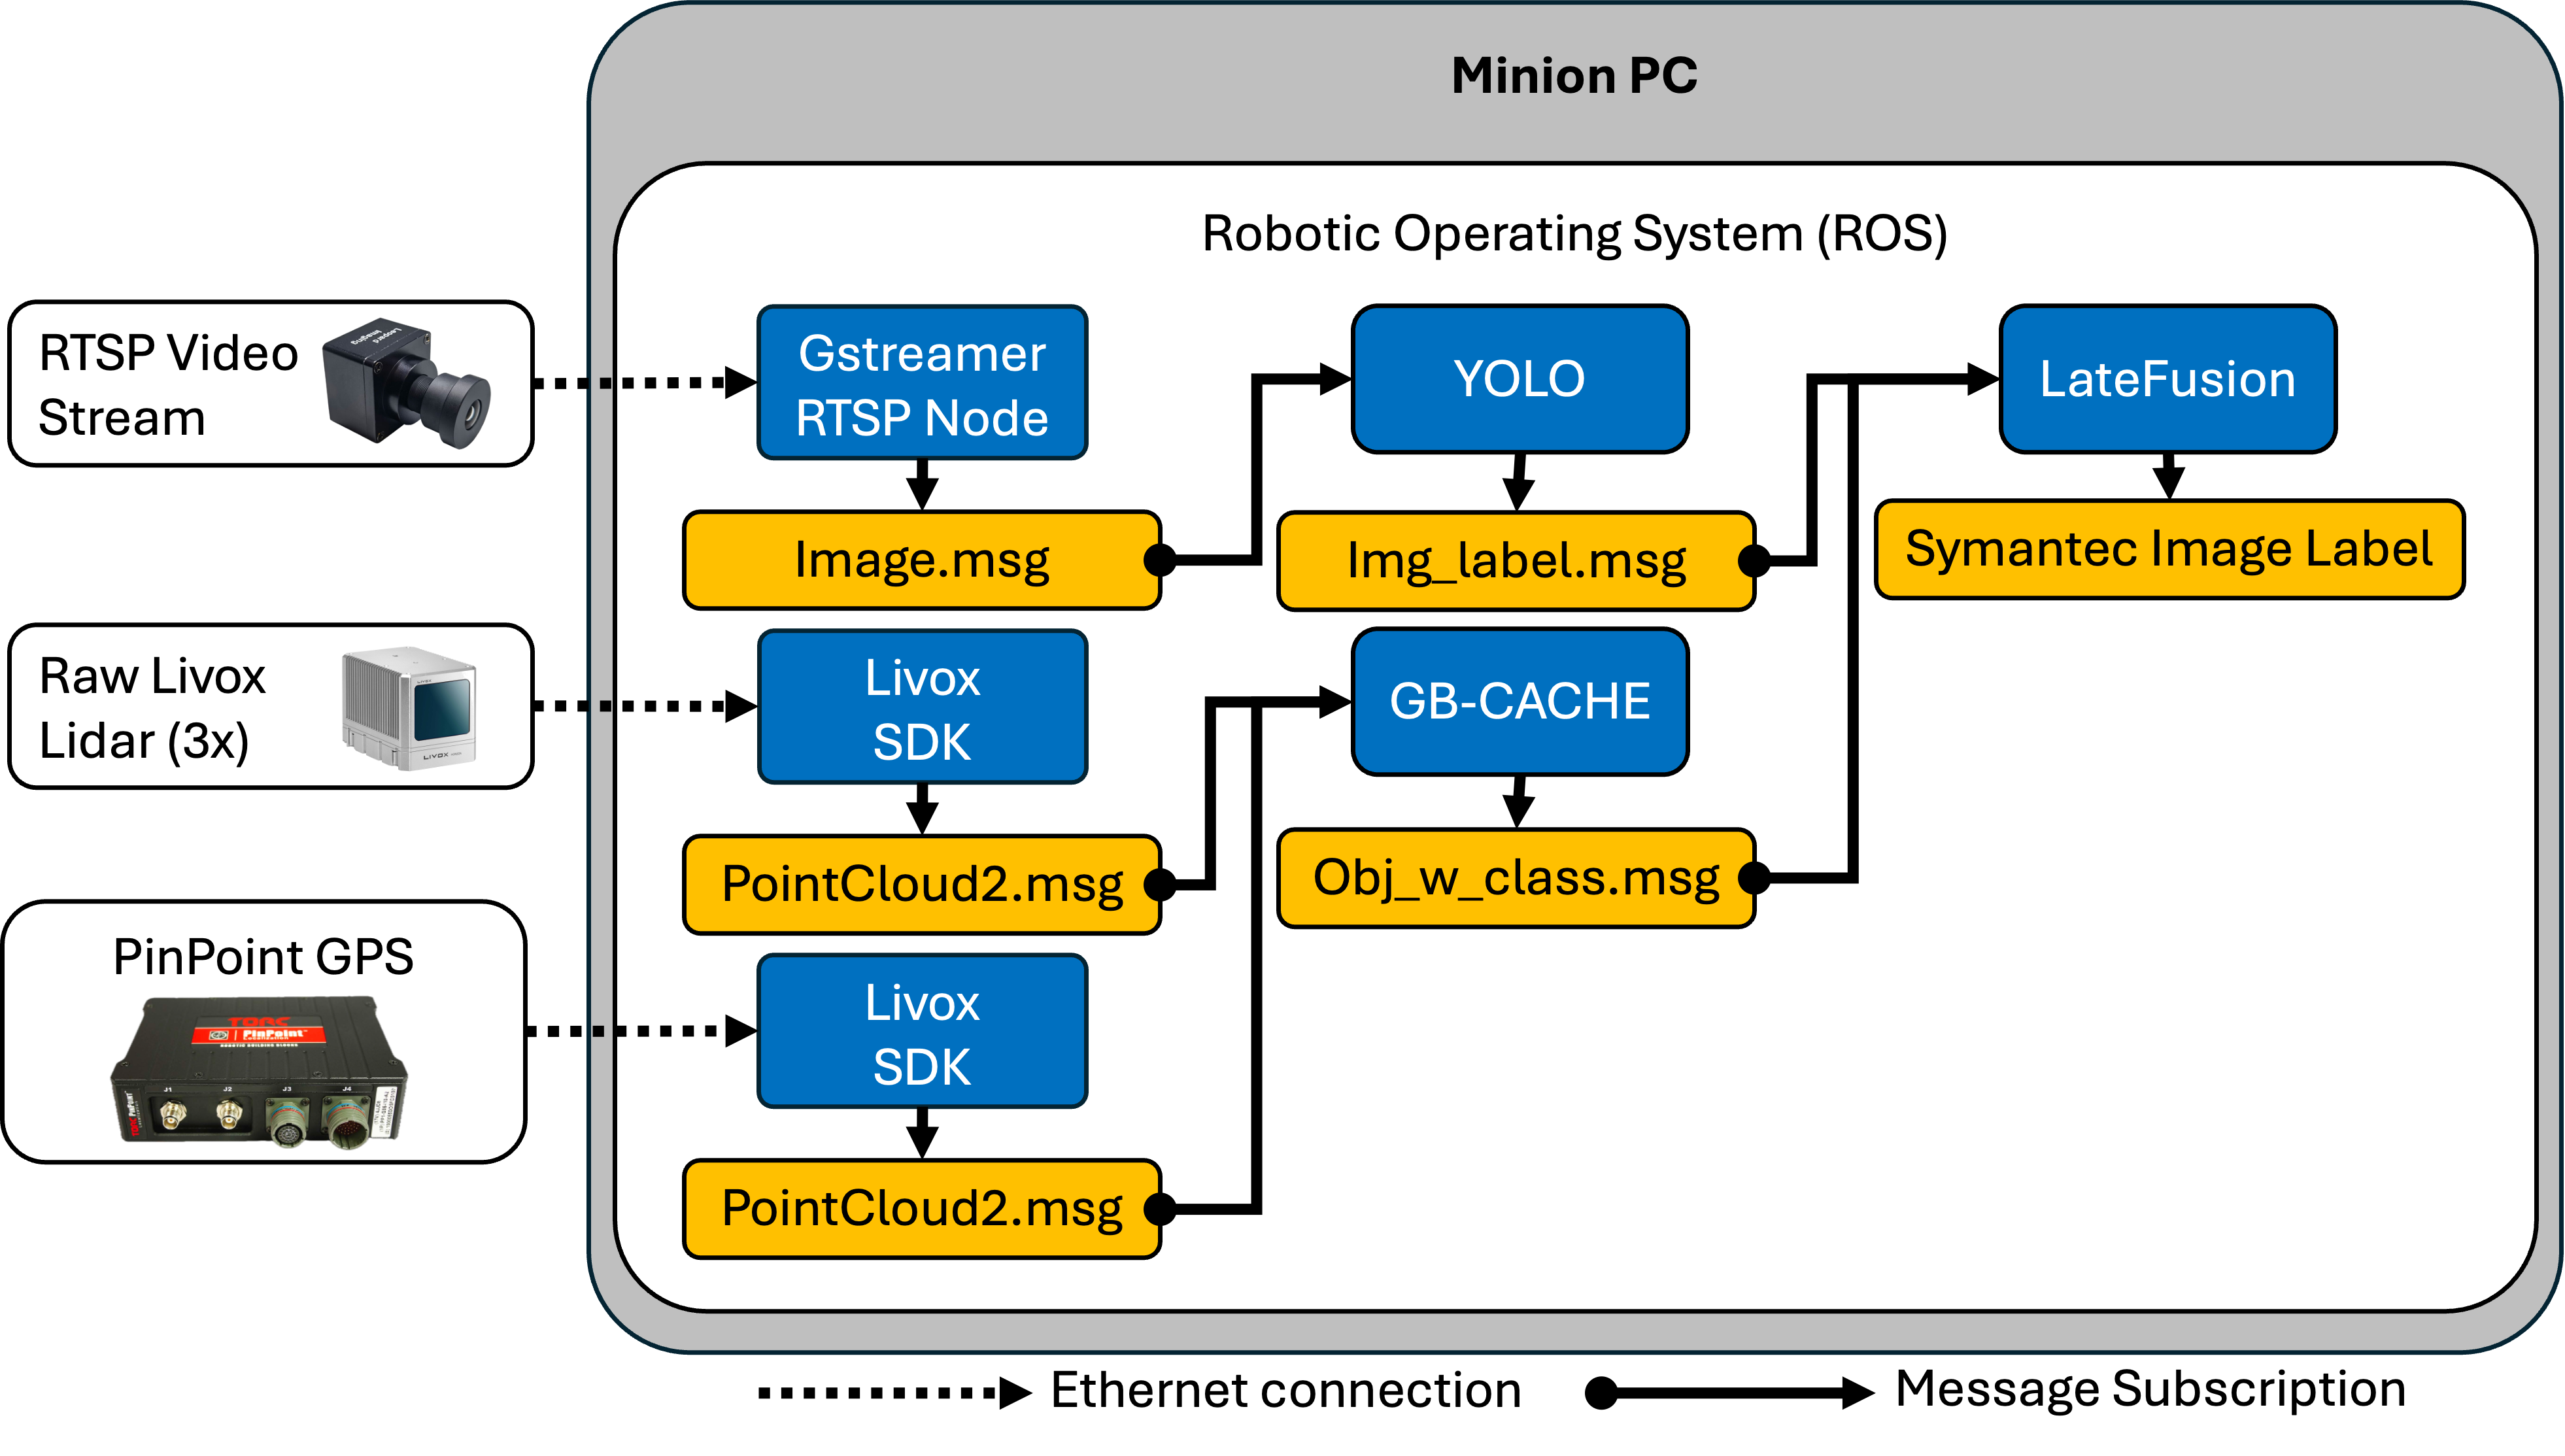
\includegraphics[width=0.95\linewidth]{Images/ros.png}
    \caption{Software architecture used to acquire synchronized LiDAR, HDR video, GPS, and IMU data within the ROS 1 Noetic framework. Each node publishes time-stamped sensor messages to modality-specific topics, allowing for the raw data to be played back with accurate timing.}
    \label{fig:ros}
\end{figure}



%%%%%%%%%%%%%%%%%%%%%%%%%%%%%%%%%%%%%%%%%%%%%%%%%%%%%%%%%%%%%%
\subsection{Data Collection Overview}
\label{sec:data_overview}

The data collection framework was deployed aboard Minion across multiple field days before, during, and after the RobotX Competition, producing the complete dataset used in this research.
A total of 122 ROS bag files were recorded over 13 collection days,  containing more than 52 million sensor messages and 3.67 hours of synchronized data.
Across all campaigns, the dataset includes approximately 132,000 camera frames and 66,000 LiDAR scans, corresponding to an average of about 10,000 frames per collection day.
Tables \ref{tab:rosbag_stats} and \ref{tab:obj_class_dets} aggregate these statistics.  
HDR messages correspond to the total number of image-topic messages recorded, and LiDAR message counts can be estimated as the total recorded duration multiplied by 300 messages per second (three sensors operating at 100 Hz each).
Based on the total durations of recorded bagfiles, this equates to more than 3.9 million LiDAR frames per unit and more than 11 million LiDAR messages when combined.

\begin{table}[htbp]
\centering
\begin{tabular}{llrrr}
\hline
\multicolumn{2}{c}{Collection Period} & Bags & HDR Messages & Seconds \\
\hline
\hline
Competition Training & Sep 22 - Oct 26, 2024 & 29 & 8,408,242 & 2,145 \\
RobotX Competition & Nov 3 - Nov 9, 2024 & 62 & 33,336,777 & 8,026 \\
Summer 2025  & May 29, 2025 & 31 & 10,488,090 & 3,010 \\
\hline
\textbf{Total} & \textbf{---} & \textbf{122} & \textbf{52,233,109} & \textbf{13,181} \\
\hline
\end{tabular}
\caption{Overall data collection statistics for each campaign, showing the number of ROS bag files, total recorded messages, and total recording duration in seconds.}
\label{tab:rosbag_stats}
\end{table}

Peak collection occurred during November 2024 in preparation for the Maritime RobotX Challenge, with additional data gathered during Summer 2025 to expand environmental variety.  
Data collection was limited to favorable weather conditions to ensure team and equipment safety. 
All sessions were conducted under calm seas, low winds, and generally clear or partly cloudy skies, with no recordings made during inclement or low-visibility conditions.
Each recording included synchronized data from three Livox Horizon LiDARs  (\texttt{/livox/lidar\_front}, \texttt{/livox/lidar\_port}, and  \texttt{/livox/lidar\_starboard}), one Leopard Imaging HDR camera publishing  \texttt{/camera/image} and \texttt{/camera/info}, and the IMU and GPS topics defining the  \texttt{map\_to\_base\_link} and \texttt{base\_link\_to\_sensor} transforms.
For clarity, topic and sensor identifiers are presented here using descriptive names (e.g., \texttt{/livox/lidar\_front}), whereas the original recorded topics used serial-number-based identifiers corresponding to each LiDAR unit.


\begin{table}[ht]
\centering
\begin{tabular}{llll}
\hline
\multicolumn{4}{c}{Total Object Detections by Class}\\
\hline
\hline
Class & Class       & Num. Samples & Unique Objs \\
1     & Tall Buoy   & 266381       & 730         \\
2     & A2 Buoy     & 83583        & 674         \\
3     & A3 Buoy     & 69559        & 803         \\
5     & Light Tower & 13171        & 48          \\
7     & Kayak       & 1624         & 39          \\
8     & Jon Boat    & 7543         & 171         \\
11    & Sailboat    & 7617         & 140  \\      
\hline
\end{tabular}
\caption{Total object detections and unique object counts for each labeled maritime class within the processed dataset.}
\label{tab:obj_class_dets}
\end{table}

Unique objects correspond to persistent object IDs assigned by the mapping system, as described in Section~\ref{gbcache}.

\begin{table}[ht]
\centering
\begin{tabular}{cllcc}
\hline
Legacy ID & Legacy Label & YOLO Label & LiDAR Label  & Included \\
\hline
1  & Tall Buoy          & Tall Buoy              & Tall Buoy          & Yes \\
2  & A2 Buoy            & Round Buoy (merged)    & A2 Buoy            & Yes \\
3  & A3 Buoy            & Round Buoy (merged)    & A3 Buoy            & Yes \\
4  & A5  Buoy           & —                      & —                  & - \\
5  & Light Tower        & Light Tower            & Light Tower        & Yes \\
6  & Dock               & —                      & —                  & - \\
7  & Power Boat         & Jon Boat               & Jon Boat           & Yes \\
8  & Sailboat           & Sailboat               & Sailboat           & Yes \\
9  & Kayak              & —                      & —                  & - \\
10 & UAV\_SR    & —                      & —                  & - \\
11 & UAV\_Rep   & —                      & —                  & - \\
\hline
\end{tabular}
\caption{Modality-aware class mapping. YOLO merges A2/A3 into \emph{Round Buoy} because a single monocular image does not provide absolute scale; LiDAR retains A2 and A3 as distinct classes due to direct range measurements enabling size-based separation.}
\label{tab:class_map}
\end{table}

Metadata from each bagfile and associated video files, including topic names, message counts, and timestamps, were compiled into an SQLite3 database to support efficient indexing, retrieval, and temporal alignment tasks outlined in section~\ref{time_sync_cam}.
This dataset structure provides the foundation for the evaluation results presented in Chapter~\ref{realtime_object_detection}.

% %%%%%%%%%%%%%%%%%%%%%%%%%%%%%%%%%%%%%%%%%%%%%%%%%%%%%%%%%%%%%%
% \subsection{Data Organization and Processing}
% \label{sec:data_organization}

% The recorded dataset consists of multiple ROS topics operating at distinct rates. 
% The three Livox LiDAR sensors published point-cloud data at 100~Hz, the HDR camera produced image messages at 5~Hz, 
% and the combined GPS/IMU localization topics updated at approximately 5~Hz. 
% These asynchronous data streams were recorded concurrently into ROS bag files during field operations, forming the complete dataset used for subsequent analysis.

% All data were later reprocessed within ROS for operational testing and analysis. 
% Metadata from each bag file, including topic names, message counts, and timestamps, was extracted into an SQLite3 database 
% to support efficient indexing, retrieval, and temporal alignment tasks outlined in section~\ref{time_sync_cam}.
% This dataset structure provides the foundation for the training and evaluation results presented in Chapters~\ref{yolo} and~\ref{gbcache}. 
% The organization described here ensures that the models discussed in those chapters operate on a consistent, time-synchronized dataset, 
% allowing direct comparison of performance between the vision-only YOLO framework and the LiDAR-based GB-CACHE method.

% \paragraph{Temporal Synchronization}  
% Detailed discussion of temporal alignment and clock drift correction is provided in Section~\ref{time_sync_cam}. 
% Briefly, image and LiDAR frames were associated based on their recorded timestamps, ensuring that each pair represented 
% the closest available acquisition times within a latency bound of 50~ms.

% \paragraph{Spatial Registration}  
% Spatial alignment of LiDAR data to the camera frame use the extrinsic calibration derived in Section~\ref{sec:camera-lidar_results}. 
% Because the GPS/IMU topics operated at a lower rate than the LiDAR, the \texttt{robot\-localization} package within ROS interpolated position and heading between consecutive 5~Hz updates to generate intermediate pose estimates at 100~Hz. 
% These interpolated poses ensured each LiDAR scan was transformed using a temporally consistent platform orientation and position.


% %%%%%%%%%%%%%%%%%%%%%%%%%%%%%%%%%%%%%%%%%%%%%%%%%%%%%%%%%%%%%%
% \subsection{Dataset Construction for Machine Learning}
% \label{sec:dataset_construction}

% The processed dataset forms the basis for training and validating the vision and fusion models described in Chapters \ref{yolo} and \ref{gbcache}.  
% The dataset contains labeled maritime object classes, including navigation buoys, docks, vessels, and channel markers.  
% Each object instance includes a cropped RGB image (2880 × 1860 resized to 640 × 640 for network input), a corresponding LiDAR point subset in PCD format, a YOLO label file with normalized bounding boxes, and associated metadata such as timestamp, GPS pose, and lighting condition.

% The final YOLO training dataset consisted of 543 labeled images for training, 158 for validation, and 77 for testing. 
% Across all splits, the dataset contained 1,934 labeled objects with an average of 2.5 bounding boxes per image. 
% The class distribution was moderately imbalanced, with sailboats representing approximately 60\% of annotations, 
% followed by jon boats ($16$\%), tall buoys ($12$\%), light towers ($11$\%), and minor representation of round buoys and A3 markers ($<2$\%). 
% This class composition reflects the real-world frequency of visible maritime targets encountered during data collection.
% Training, validation, and test splits follow a 70 / 20 / 10 ratio, stratified by date to prevent temporal leakage between sets.

% The five YOLO class labels, tall\_buoy, round\_buoy, light\_tower, jon\_boat, and sailboat, correspond directly to the maritime object categories summarized in Tables~\ref{tab:obj_class_dets} and~\ref{tab:class_map}, with one key distinction. 
% While the LiDAR-based detection framework differentiates between A2- and A3-sized buoys as separate classes, these were combined into a single round\_buoy category for YOLO training because visual appearance alone does not reliably convey scale or distance. 
% As a result, the LiDAR models operate on six classes, whereas the YOLO models use five, excluding kayaks from both datasets due to insufficient representation for robust training.

%%%%%%%%%%%%%%%%%%%%%%%%%%%%%%%%%%%%%%%%%%%%%%%%%%%%%%%%%%%%%%
% \subsection{GB-CACHE Training Dataset}
% \label{sec:gbcache_training_data}

% \begin{figure}[htbp]
%     \centering
%     \includegraphics[width=0.9\linewidth]{Images/dataset_pipeline.pdf}
%     \caption{Processing pipeline from raw ROS bags to labeled training dataset.}
%     \label{fig:dataset_pipeline}
% \end{figure}

% This dataset structure provides the foundation for the training and evaluation results presented in Chapters~\ref{yolo} and~\ref{gbcache}. 
% The organization described here ensures that the models discussed in those chapters operate on a consistent, time-synchronized dataset, 
% allowing direct comparison of performance between the vision-only YOLO framework and the LiDAR-based GB-CACHE method.



%%%%%%%%%%%%%%%%%%%%%%%%%%%%%%%%%%%%%%%%%%%%%%%%%%%%%%%%%%%%%%%%%%%%
%%%%%%%%%%%%%%%%%%%%%%%%%%%%%%%%%%%%%%%%%%%%%%%%%%%%%%%%%%%%%%%%%%%%
%%%%%%%%%%%%%%%%%%%%%%%%%%%%%%%%%%%%%%%%%%%%%%%%%%%%%%%%%%%%%%%%%%%%

\end{document}
